\documentclass[]{article}
\usepackage[T1]{fontenc}
\usepackage{lmodern}
\usepackage{amssymb,amsmath}
\usepackage{ifxetex,ifluatex}
\usepackage{fixltx2e} % provides \textsubscript
% Set line spacing
% use upquote if available, for straight quotes in verbatim environments
\IfFileExists{upquote.sty}{\usepackage{upquote}}{}
\ifnum 0\ifxetex 1\fi\ifluatex 1\fi=0 % if pdftex
  \usepackage[utf8]{inputenc}
\else % if luatex or xelatex
  \ifxetex
    \usepackage{mathspec}
    \usepackage{xltxtra,xunicode}
  \else
    \usepackage{fontspec}
  \fi
  \defaultfontfeatures{Mapping=tex-text,Scale=MatchLowercase}
  \newcommand{\euro}{€}
\fi
% use microtype if available
\IfFileExists{microtype.sty}{\usepackage{microtype}}{}
\usepackage[margin=1in]{geometry}
\usepackage{color}
\usepackage{fancyvrb}
\newcommand{\VerbBar}{|}
\newcommand{\VERB}{\Verb[commandchars=\\\{\}]}
\DefineVerbatimEnvironment{Highlighting}{Verbatim}{commandchars=\\\{\}}
% Add ',fontsize=\small' for more characters per line
\usepackage{framed}
\definecolor{shadecolor}{RGB}{248,248,248}
\newenvironment{Shaded}{\begin{snugshade}}{\end{snugshade}}
\newcommand{\KeywordTok}[1]{\textcolor[rgb]{0.13,0.29,0.53}{\textbf{{#1}}}}
\newcommand{\DataTypeTok}[1]{\textcolor[rgb]{0.13,0.29,0.53}{{#1}}}
\newcommand{\DecValTok}[1]{\textcolor[rgb]{0.00,0.00,0.81}{{#1}}}
\newcommand{\BaseNTok}[1]{\textcolor[rgb]{0.00,0.00,0.81}{{#1}}}
\newcommand{\FloatTok}[1]{\textcolor[rgb]{0.00,0.00,0.81}{{#1}}}
\newcommand{\CharTok}[1]{\textcolor[rgb]{0.31,0.60,0.02}{{#1}}}
\newcommand{\StringTok}[1]{\textcolor[rgb]{0.31,0.60,0.02}{{#1}}}
\newcommand{\CommentTok}[1]{\textcolor[rgb]{0.56,0.35,0.01}{\textit{{#1}}}}
\newcommand{\OtherTok}[1]{\textcolor[rgb]{0.56,0.35,0.01}{{#1}}}
\newcommand{\AlertTok}[1]{\textcolor[rgb]{0.94,0.16,0.16}{{#1}}}
\newcommand{\FunctionTok}[1]{\textcolor[rgb]{0.00,0.00,0.00}{{#1}}}
\newcommand{\RegionMarkerTok}[1]{{#1}}
\newcommand{\ErrorTok}[1]{\textbf{{#1}}}
\newcommand{\NormalTok}[1]{{#1}}
\usepackage{graphicx}
% Redefine \includegraphics so that, unless explicit options are
% given, the image width will not exceed the width of the page.
% Images get their normal width if they fit onto the page, but
% are scaled down if they would overflow the margins.
\makeatletter
\def\ScaleIfNeeded{%
  \ifdim\Gin@nat@width>\linewidth
    \linewidth
  \else
    \Gin@nat@width
  \fi
}
\makeatother
\let\Oldincludegraphics\includegraphics
{%
 \catcode`\@=11\relax%
 \gdef\includegraphics{\@ifnextchar[{\Oldincludegraphics}{\Oldincludegraphics[width=\ScaleIfNeeded]}}%
}%
\ifxetex
  \usepackage[setpagesize=false, % page size defined by xetex
              unicode=false, % unicode breaks when used with xetex
              xetex]{hyperref}
\else
  \usepackage[unicode=true]{hyperref}
\fi
\hypersetup{breaklinks=true,
            bookmarks=true,
            pdfauthor={Gitanshu Munjal},
            pdftitle={Problem Set 1},
            colorlinks=true,
            citecolor=blue,
            urlcolor=blue,
            linkcolor=magenta,
            pdfborder={0 0 0}}
\urlstyle{same}  % don't use monospace font for urls
\setlength{\parindent}{0pt}
\setlength{\parskip}{6pt plus 2pt minus 1pt}
\setlength{\emergencystretch}{3em}  % prevent overfull lines
\setcounter{secnumdepth}{0}

%%% Change title format to be more compact
\usepackage{titling}
\setlength{\droptitle}{-2em}
  \title{Problem Set 1}
  \pretitle{\vspace{\droptitle}\centering\huge}
  \posttitle{\par}
  \author{Gitanshu Munjal}
  \preauthor{\centering\large\emph}
  \postauthor{\par}
  \predate{\centering\large\emph}
  \postdate{\par}
  \date{Saturday, April 11, 2015}




\begin{document}

\maketitle


\section{Problem 1}\label{problem-1}

\subsection{Calculate the allele frequenies for each
locus.}\label{calculate-the-allele-frequenies-for-each-locus.}

I define an R function to calculate allele frequencies for a bi-allelic
locus given genotype frequencies. When provided genotype frequencies in
the order (homozygous1, heterozygous, homozygous2), the function returns
frequency of allele1, frequency of allele2, and 1-frequency of allele1
(added to double check calc. allele 2 frequency). I recycle this
function for later questions in the assignment.

\begin{Shaded}
\begin{Highlighting}[]
\NormalTok{################################################}
\CommentTok{# Allele Frequencies}
\NormalTok{################################################}

\NormalTok{allelefrequency <-}\StringTok{ }\NormalTok{function(ho1,het,ho2)\{}
                                  \NormalTok{a1 <-}\StringTok{ }\NormalTok{(}\DecValTok{2}\NormalTok{*ho1 +}\StringTok{ }\NormalTok{het)/(}\DecValTok{2}\NormalTok{*(ho1+het+ho2));}
                                  \NormalTok{a2 <-}\StringTok{ }\NormalTok{(}\DecValTok{2}\NormalTok{*ho2 +}\StringTok{ }\NormalTok{het)/(}\DecValTok{2}\NormalTok{*(ho1+het+ho2));}
                                  \NormalTok{a2c <-}\StringTok{ }\DecValTok{1}\NormalTok{-a1;}
                                  \NormalTok{freqs <-}\StringTok{ }\KeywordTok{c}\NormalTok{(}\StringTok{"allele1"}\NormalTok{=a1,}\StringTok{"allele2"}\NormalTok{=a2,}\StringTok{"1-allele1"}\NormalTok{=a2c)}
                                  \KeywordTok{return}\NormalTok{(freqs)}
                   \NormalTok{\}}
  

\CommentTok{#Locus1}
\NormalTok{ho1 <-}\StringTok{ }\NormalTok{cc <-}\StringTok{ }\DecValTok{47}     \CommentTok{# allele1 = c}
\NormalTok{het <-}\StringTok{ }\NormalTok{ct <-}\StringTok{ }\DecValTok{18}
\NormalTok{ho2 <-}\StringTok{ }\NormalTok{tt <-}\StringTok{ }\DecValTok{35}     \CommentTok{# allele2 = t}
\KeywordTok{allelefrequency}\NormalTok{(ho1,het,ho2)}
\end{Highlighting}
\end{Shaded}

\begin{verbatim}
##   allele1   allele2 1-allele1 
##      0.56      0.44      0.44
\end{verbatim}

\textbf{So,the frequency of the C and T alleles at Locus 1 are 0.56 and
0.44 respectively.}

\begin{Shaded}
\begin{Highlighting}[]
\CommentTok{#Locus2}
\NormalTok{ho1 <-}\StringTok{ }\NormalTok{aa <-}\StringTok{ }\DecValTok{50}     \CommentTok{# allele1 = a}
\NormalTok{het <-}\StringTok{ }\NormalTok{ag <-}\StringTok{ }\DecValTok{42}
\NormalTok{ho2 <-}\StringTok{ }\NormalTok{gg <-}\StringTok{ }\DecValTok{8}      \CommentTok{# allele2 = g}
\KeywordTok{allelefrequency}\NormalTok{(ho1,het,ho2)}
\end{Highlighting}
\end{Shaded}

\begin{verbatim}
##   allele1   allele2 1-allele1 
##      0.71      0.29      0.29
\end{verbatim}

\textbf{So,the frequency of the A and G alleles at Locus 2 are 0.56 and
0.44 respectively.}\\

\begin{center}
\line(1,0){250}
\end{center}

\subsection{What is the expected heterozygosity for each locus given the
allele
frequencies?}\label{what-is-the-expected-heterozygosity-for-each-locus-given-the-allele-frequencies}

I define a function to return the expected frequency of heterozygous
genotypes as 2pq when allele frequencies are p and q.

\begin{Shaded}
\begin{Highlighting}[]
\NormalTok{################################################}
\CommentTok{# Expected heterozygosity}
\NormalTok{################################################}

\NormalTok{ehetero <-}\StringTok{ }\NormalTok{function(p,q)\{}\DecValTok{2}\NormalTok{*p*q\}}

\CommentTok{#Locus1}
\KeywordTok{ehetero}\NormalTok{(}\FloatTok{0.56}\NormalTok{,}\FloatTok{0.44}\NormalTok{)}
\end{Highlighting}
\end{Shaded}

\begin{verbatim}
## [1] 0.4928
\end{verbatim}

\begin{Shaded}
\begin{Highlighting}[]
\CommentTok{#Locus2}
\KeywordTok{ehetero}\NormalTok{(}\FloatTok{0.71}\NormalTok{,}\FloatTok{0.29}\NormalTok{)}
\end{Highlighting}
\end{Shaded}

\begin{verbatim}
## [1] 0.4118
\end{verbatim}

\textbf{So, expected frequency of heterozygous genotypes at Locus 1 and
Locus 2 are 0.4928 and 0.411 respectively.}

\begin{center}
\line(1,0){250}
\end{center}

\subsection{Does the population significantly deviate from
Hardy-Weinberg Equilibrium (HWE) at each
locus?}\label{does-the-population-significantly-deviate-from-hardy-weinberg-equilibrium-hwe-at-each-locus}

\begin{Shaded}
\begin{Highlighting}[]
\NormalTok{################################################}
\CommentTok{# Test for Hardy-Weinberg Equilibrium (HWE)}
\NormalTok{################################################}

\CommentTok{#Locus1}
\CommentTok{#Observed data (genotype counts)}
\NormalTok{occ <-}\StringTok{ }\DecValTok{47}     \CommentTok{# allele1 = c}
\NormalTok{oct <-}\StringTok{ }\DecValTok{18}
\NormalTok{ott <-}\StringTok{ }\DecValTok{35}     \CommentTok{# allele2 = t}
\NormalTok{total <-}\StringTok{ }\NormalTok{occ+oct+ott}

\CommentTok{#Expected frequency (under HWE)}
\NormalTok{p <-}\StringTok{ }\KeywordTok{as.numeric}\NormalTok{(}\KeywordTok{allelefrequency}\NormalTok{(occ,oct,ott)[}\DecValTok{1}\NormalTok{])}
\NormalTok{q <-}\StringTok{ }\KeywordTok{as.numeric}\NormalTok{(}\KeywordTok{allelefrequency}\NormalTok{(occ,oct,ott)[}\DecValTok{2}\NormalTok{])}

\CommentTok{#Expected genotype counts}
\NormalTok{ecc <-}\StringTok{ }\NormalTok{p^}\DecValTok{2} \NormalTok{*}\StringTok{ }\NormalTok{total}
\NormalTok{ect <-}\StringTok{ }\DecValTok{2}\NormalTok{*p*q *}\StringTok{ }\NormalTok{total}
\NormalTok{ett <-}\StringTok{ }\NormalTok{q^}\DecValTok{2} \NormalTok{*}\StringTok{ }\NormalTok{total}
\KeywordTok{c}\NormalTok{(}\StringTok{"ecc"}\NormalTok{=ecc,}\StringTok{"ect"}\NormalTok{=ect,}\StringTok{"ett"}\NormalTok{=ett)}
\end{Highlighting}
\end{Shaded}

\begin{verbatim}
##   ecc   ect   ett 
## 31.36 49.28 19.36
\end{verbatim}

\begin{Shaded}
\begin{Highlighting}[]
\CommentTok{#Matrix containing observed and expected data}
\NormalTok{hwedat <-}\StringTok{ }\KeywordTok{matrix}\NormalTok{(}\OtherTok{NA}\NormalTok{,}\DecValTok{3}\NormalTok{,}\DecValTok{3}\NormalTok{)}
\KeywordTok{colnames}\NormalTok{(hwedat) <-}\StringTok{ }\KeywordTok{c}\NormalTok{(}\StringTok{"observed"}\NormalTok{,}\StringTok{"expected"}\NormalTok{,}\StringTok{"(o-e)^2/e"}\NormalTok{)}
\KeywordTok{rownames}\NormalTok{(hwedat) <-}\StringTok{ }\KeywordTok{c}\NormalTok{(}\StringTok{"cc"}\NormalTok{,}\StringTok{"ct"}\NormalTok{,}\StringTok{"tt"}\NormalTok{)}
\NormalTok{hwedat[,}\DecValTok{1}\NormalTok{] <-}\StringTok{ }\KeywordTok{c}\NormalTok{(occ,oct,ott)}
\NormalTok{hwedat[,}\DecValTok{2}\NormalTok{] <-}\StringTok{ }\KeywordTok{c}\NormalTok{(ecc,ect,ett)}
\NormalTok{obs <-}\StringTok{ }\NormalTok{hwedat[,}\DecValTok{1}\NormalTok{]}
\NormalTok{exp <-}\StringTok{ }\NormalTok{hwedat[,}\DecValTok{2}\NormalTok{]}
\NormalTok{hwedat[,}\DecValTok{3}\NormalTok{] <-}\StringTok{ }\NormalTok{((obs -}\StringTok{ }\NormalTok{exp)^}\DecValTok{2}\NormalTok{)/exp}
\NormalTok{hwedat}
\end{Highlighting}
\end{Shaded}

\begin{verbatim}
##    observed expected (o-e)^2/e
## cc       47    31.36  7.800051
## ct       18    49.28 19.854675
## tt       35    19.36 12.634793
\end{verbatim}

\begin{Shaded}
\begin{Highlighting}[]
\CommentTok{#Chi-square and p-value}
\NormalTok{chisq <-}\StringTok{ }\KeywordTok{sum}\NormalTok{(hwedat[,}\DecValTok{3}\NormalTok{])}
\NormalTok{chisq                               }\CommentTok{#chi-squared value}
\end{Highlighting}
\end{Shaded}

\begin{verbatim}
## [1] 40.28952
\end{verbatim}

\begin{Shaded}
\begin{Highlighting}[]
\KeywordTok{pchisq}\NormalTok{(chisq,}\DataTypeTok{df=}\DecValTok{1}\NormalTok{,}\DataTypeTok{lower.tail=}\OtherTok{FALSE}\NormalTok{) }\CommentTok{#p-value}
\end{Highlighting}
\end{Shaded}

\begin{verbatim}
## [1] 2.189805e-10
\end{verbatim}

Indeed, \textbf{the population significantly deviates from HWE at Locus
1} at the 95\% confidence level.

\begin{Shaded}
\begin{Highlighting}[]
\CommentTok{#Locus2}
\CommentTok{#Observed data (genotype counts)}
\NormalTok{oaa <-}\StringTok{ }\DecValTok{50}     \CommentTok{# allele1 = a}
\NormalTok{oag <-}\StringTok{ }\DecValTok{42}
\NormalTok{ogg <-}\StringTok{ }\DecValTok{8}     \CommentTok{# allele2 = g}
\NormalTok{total <-}\StringTok{ }\NormalTok{oaa+oag+ogg}

\CommentTok{#Expected frequency (under HWE)}
\NormalTok{p <-}\StringTok{ }\KeywordTok{as.numeric}\NormalTok{(}\KeywordTok{allelefrequency}\NormalTok{(oaa,oag,ogg)[}\DecValTok{1}\NormalTok{])}
\NormalTok{q <-}\StringTok{ }\KeywordTok{as.numeric}\NormalTok{(}\KeywordTok{allelefrequency}\NormalTok{(oaa,oag,ogg)[}\DecValTok{2}\NormalTok{])}

\CommentTok{#Expected genotype counts}
\NormalTok{eaa <-}\StringTok{ }\NormalTok{p^}\DecValTok{2} \NormalTok{*}\StringTok{ }\NormalTok{total}
\NormalTok{eag <-}\StringTok{ }\DecValTok{2}\NormalTok{*p*q *}\StringTok{ }\NormalTok{total}
\NormalTok{egg <-}\StringTok{ }\NormalTok{q^}\DecValTok{2} \NormalTok{*}\StringTok{ }\NormalTok{total}
\KeywordTok{c}\NormalTok{(}\StringTok{"eaa"}\NormalTok{=eaa,}\StringTok{"eag"}\NormalTok{=eag,}\StringTok{"egg"}\NormalTok{=egg)}
\end{Highlighting}
\end{Shaded}

\begin{verbatim}
##   eaa   eag   egg 
## 50.41 41.18  8.41
\end{verbatim}

\begin{Shaded}
\begin{Highlighting}[]
\NormalTok{hwedat <-}\StringTok{ }\KeywordTok{matrix}\NormalTok{(}\OtherTok{NA}\NormalTok{,}\DecValTok{3}\NormalTok{,}\DecValTok{3}\NormalTok{)}
\KeywordTok{colnames}\NormalTok{(hwedat) <-}\StringTok{ }\KeywordTok{c}\NormalTok{(}\StringTok{"observed"}\NormalTok{,}\StringTok{"expected"}\NormalTok{,}\StringTok{"(o-e)^2/e"}\NormalTok{)}
\KeywordTok{rownames}\NormalTok{(hwedat) <-}\StringTok{ }\KeywordTok{c}\NormalTok{(}\StringTok{"aa"}\NormalTok{,}\StringTok{"ag"}\NormalTok{,}\StringTok{"gg"}\NormalTok{)}
\NormalTok{hwedat[,}\DecValTok{1}\NormalTok{] <-}\StringTok{ }\KeywordTok{c}\NormalTok{(oaa,oag,ogg)}
\NormalTok{hwedat[,}\DecValTok{2}\NormalTok{] <-}\StringTok{ }\KeywordTok{c}\NormalTok{(eaa,eag,egg)}
\NormalTok{obs <-}\StringTok{ }\NormalTok{hwedat[,}\DecValTok{1}\NormalTok{]}
\NormalTok{exp <-}\StringTok{ }\NormalTok{hwedat[,}\DecValTok{2}\NormalTok{]}
\NormalTok{hwedat[,}\DecValTok{3}\NormalTok{] <-}\StringTok{ }\NormalTok{((obs -}\StringTok{ }\NormalTok{exp)^}\DecValTok{2}\NormalTok{)/exp}
\NormalTok{hwedat}
\end{Highlighting}
\end{Shaded}

\begin{verbatim}
##    observed expected   (o-e)^2/e
## aa       50    50.41 0.003334656
## ag       42    41.18 0.016328315
## gg        8     8.41 0.019988109
\end{verbatim}

\begin{Shaded}
\begin{Highlighting}[]
\NormalTok{chisq <-}\StringTok{ }\KeywordTok{sum}\NormalTok{(hwedat[,}\DecValTok{3}\NormalTok{])}
\NormalTok{chisq                               }\CommentTok{#chi-squared value}
\end{Highlighting}
\end{Shaded}

\begin{verbatim}
## [1] 0.03965108
\end{verbatim}

\begin{Shaded}
\begin{Highlighting}[]
\KeywordTok{pchisq}\NormalTok{(chisq,}\DataTypeTok{df=}\DecValTok{1}\NormalTok{,}\DataTypeTok{lower.tail=}\OtherTok{FALSE}\NormalTok{) }\CommentTok{#p-value}
\end{Highlighting}
\end{Shaded}

\begin{verbatim}
## [1] 0.8421643
\end{verbatim}

At the 95\% confidence level, \textbf{the population does not
significantly deviate from HWE at Locus 2.}

\begin{center}
\line(1,0){250}
\end{center}

\subsection{What are two possible reasons a population would deviate
from
HWE?}\label{what-are-two-possible-reasons-a-population-would-deviate-from-hwe}

\begin{enumerate}
\def\labelenumi{(\arabic{enumi})}
\itemsep1pt\parskip0pt\parsep0pt
\item
  Non-random mating
\item
  Migration (I/E-mmigration)

  \begin{center}
  \line(1,0){250}
  \end{center}
\end{enumerate}

\pagebreak

\section{Problem 2}\label{problem-2}

\subsection{How many of each haplotype were definitively observed in
this
population?}\label{how-many-of-each-haplotype-were-definitively-observed-in-this-population}

All genotypes except the CTAG double heterozygote contribute towardss
the observed haplotypes. Double homozygotes contribute $2N$ haplotypes
and heterozygotes for one or the other locus contribute N haplotypes
where $N$ is the number of individuals with the haplotype under
consideration.

\begin{Shaded}
\begin{Highlighting}[]
\NormalTok{################################################}
\CommentTok{# Definitively Observed Haplotypes}
\NormalTok{################################################}

\NormalTok{CA <-}\StringTok{ }\NormalTok{(}\DecValTok{2}\NormalTok{*}\DecValTok{40}\NormalTok{) +}\StringTok{ }\NormalTok{(}\DecValTok{2}\NormalTok{) +}\StringTok{ }\NormalTok{(}\DecValTok{4}\NormalTok{) }
\NormalTok{TA <-}\StringTok{ }\NormalTok{(}\DecValTok{2}\NormalTok{*}\DecValTok{8}\NormalTok{) +}\StringTok{ }\NormalTok{(}\DecValTok{2}\NormalTok{) +}\StringTok{ }\NormalTok{(}\DecValTok{22}\NormalTok{)}
\NormalTok{CG <-}\StringTok{ }\NormalTok{(}\DecValTok{2}\NormalTok{*}\DecValTok{4}\NormalTok{) +}\StringTok{ }\NormalTok{(}\DecValTok{4}\NormalTok{) +}\StringTok{ }\NormalTok{(}\DecValTok{0}\NormalTok{)}
\NormalTok{TG <-}\StringTok{ }\NormalTok{(}\DecValTok{2}\NormalTok{*}\DecValTok{4}\NormalTok{) +}\StringTok{ }\NormalTok{(}\DecValTok{22}\NormalTok{) +}\StringTok{ }\NormalTok{(}\DecValTok{0}\NormalTok{)}
\NormalTok{Total <-}\StringTok{ }\NormalTok{CA +}\StringTok{ }\NormalTok{TA +}\StringTok{ }\NormalTok{CG +}\StringTok{ }\NormalTok{TG}

\CommentTok{#Matrix of Observed Haplotypes}
\NormalTok{obsdata <-}\StringTok{ }\KeywordTok{matrix}\NormalTok{(}\OtherTok{NA}\NormalTok{,}\DecValTok{5}\NormalTok{,}\DecValTok{1}\NormalTok{)}
\KeywordTok{colnames}\NormalTok{(obsdata) <-}\StringTok{ }\KeywordTok{c}\NormalTok{(}\StringTok{"NumberObserved"}\NormalTok{)}
\KeywordTok{rownames}\NormalTok{(obsdata) <-}\StringTok{ }\KeywordTok{c}\NormalTok{(}\StringTok{"CA"}\NormalTok{,}\StringTok{"TA"}\NormalTok{,}\StringTok{"CG"}\NormalTok{,}\StringTok{"TG"}\NormalTok{,}\StringTok{"Total"}\NormalTok{)}
\NormalTok{obsdata[,}\DecValTok{1}\NormalTok{] <-}\StringTok{ }\KeywordTok{c}\NormalTok{(CA,TA,CG,TG,Total)}
\NormalTok{obsdata}
\end{Highlighting}
\end{Shaded}

\begin{verbatim}
##       NumberObserved
## CA                86
## TA                40
## CG                12
## TG                30
## Total            168
\end{verbatim}

\textbf{The above matrix shows the number of each haplotype that were
definitively observed.}

\begin{center}
\line(1,0){250}
\end{center}

\subsection{Calculate D, D', and r2 for the C-A
haplotype.}\label{calculate-d-d-and-r2-for-the-c-a-haplotype.}

I use the definitive set of observed haplotypes to calculate allele
frequencies.

\begin{Shaded}
\begin{Highlighting}[]
\NormalTok{################################################}
\CommentTok{# D, D', and r2 for the C-A haplotype}
\NormalTok{################################################}

\CommentTok{#Allele Frequencies}
\NormalTok{c <-}\StringTok{ }\NormalTok{(CA +}\StringTok{ }\NormalTok{CG) /}\StringTok{ }\NormalTok{Total}
\NormalTok{a <-}\StringTok{ }\NormalTok{(CA +}\StringTok{ }\NormalTok{TA) /}\StringTok{ }\NormalTok{Total}
\NormalTok{t <-}\StringTok{ }\NormalTok{(TA +}\StringTok{ }\NormalTok{TG) /}\StringTok{ }\NormalTok{Total}
\NormalTok{g <-}\StringTok{ }\NormalTok{(CG +}\StringTok{ }\NormalTok{TG) /}\StringTok{ }\NormalTok{Total}
\KeywordTok{c}\NormalTok{(}\StringTok{"c"}\NormalTok{=c,}\StringTok{"a"}\NormalTok{=a,}\StringTok{"t"}\NormalTok{=t,}\StringTok{"g"}\NormalTok{=g)}
\end{Highlighting}
\end{Shaded}

\begin{verbatim}
##         c         a         t         g 
## 0.5833333 0.7500000 0.4166667 0.2500000
\end{verbatim}

The allele frequencies are then used to calculate expected haplotype
frequencies

\begin{Shaded}
\begin{Highlighting}[]
\CommentTok{#Expected Haplotype Frequencies}
\NormalTok{expca <-}\StringTok{ }\NormalTok{c *}\StringTok{ }\NormalTok{a}
\NormalTok{expta <-}\StringTok{ }\NormalTok{t *}\StringTok{ }\NormalTok{a}
\NormalTok{expcg <-}\StringTok{ }\NormalTok{c *}\StringTok{ }\NormalTok{g}
\NormalTok{exptg <-}\StringTok{ }\NormalTok{t *}\StringTok{ }\NormalTok{g}
\KeywordTok{c}\NormalTok{(}\StringTok{"expca"}\NormalTok{=expca,}\StringTok{"expta"}\NormalTok{=expta,}\StringTok{"expcg"}\NormalTok{=expcg,}\StringTok{"exptg"}\NormalTok{=exptg)}
\end{Highlighting}
\end{Shaded}

\begin{verbatim}
##     expca     expta     expcg     exptg 
## 0.4375000 0.3125000 0.1458333 0.1041667
\end{verbatim}

\begin{Shaded}
\begin{Highlighting}[]
\CommentTok{#Data Matrix}
\NormalTok{parta <-}\StringTok{ }\KeywordTok{matrix}\NormalTok{(}\OtherTok{NA}\NormalTok{,}\DecValTok{5}\NormalTok{,}\DecValTok{3}\NormalTok{)}
\KeywordTok{colnames}\NormalTok{(parta) <-}\StringTok{ }\KeywordTok{c}\NormalTok{(}\StringTok{"ObservedNumber"}\NormalTok{,}\StringTok{"ObservedFrequency"}\NormalTok{,}\StringTok{"ExpectedFrequency"}\NormalTok{)}
\KeywordTok{rownames}\NormalTok{(parta) <-}\StringTok{ }\KeywordTok{c}\NormalTok{(}\StringTok{"CA"}\NormalTok{,}\StringTok{"TA"}\NormalTok{,}\StringTok{"CG"}\NormalTok{,}\StringTok{"TG"}\NormalTok{,}\StringTok{"Total"}\NormalTok{)}
\NormalTok{parta[,}\DecValTok{1}\NormalTok{] <-}\StringTok{ }\KeywordTok{c}\NormalTok{(CA,TA,CG,TG,Total)}
\NormalTok{parta[,}\DecValTok{2}\NormalTok{] <-}\StringTok{ }\NormalTok{parta[,}\DecValTok{1}\NormalTok{]/Total}
\NormalTok{parta[,}\DecValTok{3}\NormalTok{] <-}\StringTok{ }\KeywordTok{c}\NormalTok{(expca,expta,expcg,exptg,expca+expta+expcg+exptg)}
\NormalTok{parta}
\end{Highlighting}
\end{Shaded}

\begin{verbatim}
##       ObservedNumber ObservedFrequency ExpectedFrequency
## CA                86        0.51190476         0.4375000
## TA                40        0.23809524         0.3125000
## CG                12        0.07142857         0.1458333
## TG                30        0.17857143         0.1041667
## Total            168        1.00000000         1.0000000
\end{verbatim}

\begin{Shaded}
\begin{Highlighting}[]
\CommentTok{#D for C-A haplotype}
\NormalTok{obsca <-}\StringTok{ }\NormalTok{parta[}\DecValTok{1}\NormalTok{,}\DecValTok{2}\NormalTok{]}
\NormalTok{D <-}\StringTok{ }\NormalTok{obsca -}\StringTok{ }\NormalTok{expca}
\NormalTok{D}
\end{Highlighting}
\end{Shaded}

\begin{verbatim}
## [1] 0.07440476
\end{verbatim}

Thus, \textbf{D = 0.0744}

\begin{Shaded}
\begin{Highlighting}[]
\CommentTok{#D prime for C-A haplotype}
\NormalTok{Dprime <-}\StringTok{ }\NormalTok{D /}\StringTok{ }\KeywordTok{min}\NormalTok{(expcg,expta)}
\NormalTok{Dprime}
\end{Highlighting}
\end{Shaded}

\begin{verbatim}
## [1] 0.5102041
\end{verbatim}

Thus, \textbf{D' = 0.510}

\begin{Shaded}
\begin{Highlighting}[]
\CommentTok{#R squared for C-A haplotype}
\NormalTok{Rsquared <-}\StringTok{ }\NormalTok{(D^}\DecValTok{2}\NormalTok{) /}\StringTok{ }\NormalTok{(c*a*t*g)}
\NormalTok{Rsquared}
\end{Highlighting}
\end{Shaded}

\begin{verbatim}
## [1] 0.1214772
\end{verbatim}

Thus, \textbf{R$^2$ = 0.121}

\subsection{Calculate Chi-square and determine if there is significant
linkage disequilibrium (LD) at this
locus.}\label{calculate-chi-square-and-determine-if-there-is-significant-linkage-disequilibrium-ld-at-this-locus.}

We use expected and observed haplotype frequencies previously calculated
to determine expected haplotype counts assuming the total allele count
to be 168 and then compare these data with the observed data set to
determine significance of LD using a chi-squared test.

\begin{Shaded}
\begin{Highlighting}[]
\NormalTok{################################################}
\CommentTok{# Chi-square test to determine significance of LD}
\NormalTok{################################################}

\NormalTok{chisqtab <-}\StringTok{ }\KeywordTok{matrix}\NormalTok{(}\OtherTok{NA}\NormalTok{,}\DecValTok{4}\NormalTok{,}\DecValTok{3}\NormalTok{)}
\KeywordTok{colnames}\NormalTok{(chisqtab) <-}\StringTok{ }\KeywordTok{c}\NormalTok{(}\StringTok{"observed"}\NormalTok{,}\StringTok{"expected"}\NormalTok{,}\StringTok{"(o-e)^2/e"}\NormalTok{)}
\KeywordTok{rownames}\NormalTok{(chisqtab) <-}\StringTok{ }\KeywordTok{c}\NormalTok{(}\StringTok{"CA"}\NormalTok{,}\StringTok{"TA"}\NormalTok{,}\StringTok{"CG"}\NormalTok{,}\StringTok{"TG"}\NormalTok{)}
\NormalTok{obs <-}\StringTok{ }\NormalTok{chisqtab[,}\DecValTok{1}\NormalTok{] <-}\StringTok{ }\NormalTok{parta[}\DecValTok{1}\NormalTok{:}\DecValTok{4}\NormalTok{,}\DecValTok{2}\NormalTok{]*}\DecValTok{168}
\NormalTok{exp <-}\StringTok{ }\NormalTok{chisqtab[,}\DecValTok{2}\NormalTok{] <-}\StringTok{ }\NormalTok{parta[}\DecValTok{1}\NormalTok{:}\DecValTok{4}\NormalTok{,}\DecValTok{3}\NormalTok{]*}\DecValTok{168}
\NormalTok{chisqtab[,}\DecValTok{3}\NormalTok{] <-}\StringTok{ }\NormalTok{((obs -}\StringTok{ }\NormalTok{exp)^}\DecValTok{2}\NormalTok{)/exp}
\NormalTok{chisqtab}
\end{Highlighting}
\end{Shaded}

\begin{verbatim}
##    observed expected (o-e)^2/e
## CA       86     73.5  2.125850
## TA       40     52.5  2.976190
## CG       12     24.5  6.377551
## TG       30     17.5  8.928571
\end{verbatim}

\begin{Shaded}
\begin{Highlighting}[]
\NormalTok{chisq <-}\StringTok{ }\KeywordTok{sum}\NormalTok{(chisqtab[,}\DecValTok{3}\NormalTok{])}
\NormalTok{chisq                               }\CommentTok{#chi-squared value}
\end{Highlighting}
\end{Shaded}

\begin{verbatim}
## [1] 20.40816
\end{verbatim}

\begin{Shaded}
\begin{Highlighting}[]
\KeywordTok{pchisq}\NormalTok{(chisq,}\DataTypeTok{df=}\DecValTok{1}\NormalTok{,}\DataTypeTok{lower.tail=}\OtherTok{FALSE}\NormalTok{) }\CommentTok{#p-value}
\end{Highlighting}
\end{Shaded}

\begin{verbatim}
## [1] 6.256236e-06
\end{verbatim}

Indeed, \textbf{there is significant LD at this locus} at the 95\%
confience level.

\begin{center}
\line(1,0){250}
\end{center}

\pagebreak

\section{Problem 3}\label{problem-3}

\subsection{Calculate the p-value of association between genotype and
phenotype using a Chi-square test on expected and observed allele
counts.}\label{calculate-the-p-value-of-association-between-genotype-and-phenotype-using-a-chi-square-test-on-expected-and-observed-allele-counts.}

We recycle the function we defined in question 1 and use total genotype
counts (across cases and controls) to determine allele frequencies.

\begin{Shaded}
\begin{Highlighting}[]
\NormalTok{################################################}
\CommentTok{# Allele Frequencies}
\NormalTok{################################################}

\CommentTok{#Total counts}
\NormalTok{cc <-}\StringTok{ }\DecValTok{150}
\NormalTok{ca <-}\StringTok{ }\DecValTok{250}
\NormalTok{aa <-}\StringTok{ }\DecValTok{100}

\CommentTok{#Allele Frequencies}
\KeywordTok{allelefrequency}\NormalTok{(cc,ca,aa)[}\DecValTok{1}\NormalTok{] }\CommentTok{#allele1 = c ; allele2 = a)}
\end{Highlighting}
\end{Shaded}

\begin{verbatim}
## allele1 
##    0.55
\end{verbatim}

\begin{Shaded}
\begin{Highlighting}[]
\NormalTok{c <-}\StringTok{ }\KeywordTok{as.numeric}\NormalTok{(}\KeywordTok{allelefrequency}\NormalTok{(cc,ca,aa)[}\DecValTok{1}\NormalTok{])}
\NormalTok{a <-}\StringTok{ }\KeywordTok{as.numeric}\NormalTok{(}\KeywordTok{allelefrequency}\NormalTok{(cc,ca,aa)[}\DecValTok{2}\NormalTok{])}
\end{Highlighting}
\end{Shaded}

Thus, the frequencies of the C and A allele are 0.55 and 0.45
respectively. We can use these frequencies to determine the expected
allele counts for cases and controls by multiplying them each to the
number of cases and controls respectively, as follows:

\begin{Shaded}
\begin{Highlighting}[]
\CommentTok{#Matrix of observed allele counts}
\NormalTok{obsdata <-}\StringTok{ }\KeywordTok{matrix}\NormalTok{(}\OtherTok{NA}\NormalTok{,}\DecValTok{2}\NormalTok{,}\DecValTok{2}\NormalTok{)}
\KeywordTok{rownames}\NormalTok{(obsdata) <-}\StringTok{ }\KeywordTok{c}\NormalTok{(}\StringTok{"C"}\NormalTok{,}\StringTok{"A"}\NormalTok{)}
\KeywordTok{colnames}\NormalTok{(obsdata) <-}\StringTok{ }\KeywordTok{c}\NormalTok{(}\StringTok{"Cases"}\NormalTok{,}\StringTok{"Controls"}\NormalTok{)}
\NormalTok{obsdata[,}\DecValTok{1}\NormalTok{] <-}\StringTok{ }\KeywordTok{c}\NormalTok{(}\DecValTok{200}\NormalTok{,}\DecValTok{200}\NormalTok{)}
\NormalTok{obsdata[,}\DecValTok{2}\NormalTok{] <-}\StringTok{ }\KeywordTok{c}\NormalTok{(}\DecValTok{350}\NormalTok{,}\DecValTok{250}\NormalTok{)}
\NormalTok{totalcasealleles <-}\StringTok{ }\KeywordTok{sum}\NormalTok{(obsdata[,}\DecValTok{1}\NormalTok{])}
\NormalTok{totalcontrolalleles <-}\StringTok{ }\KeywordTok{sum}\NormalTok{(obsdata[,}\DecValTok{2}\NormalTok{])}
\NormalTok{obsdata}
\end{Highlighting}
\end{Shaded}

\begin{verbatim}
##   Cases Controls
## C   200      350
## A   200      250
\end{verbatim}

\pagebreak

\begin{Shaded}
\begin{Highlighting}[]
\CommentTok{#Matrix of expected allele counts}
\NormalTok{expdata <-}\StringTok{ }\KeywordTok{matrix}\NormalTok{(}\OtherTok{NA}\NormalTok{,}\DecValTok{2}\NormalTok{,}\DecValTok{2}\NormalTok{)}
\KeywordTok{rownames}\NormalTok{(expdata) <-}\StringTok{ }\KeywordTok{c}\NormalTok{(}\StringTok{"C"}\NormalTok{,}\StringTok{"A"}\NormalTok{)}
\KeywordTok{colnames}\NormalTok{(expdata) <-}\StringTok{ }\KeywordTok{c}\NormalTok{(}\StringTok{"Cases"}\NormalTok{,}\StringTok{"Controls"}\NormalTok{)}
\NormalTok{expdata[,}\DecValTok{1}\NormalTok{] <-}\StringTok{ }\KeywordTok{c}\NormalTok{(c,a)*totalcasealleles            }\CommentTok{#Expected case count}
\NormalTok{expdata[,}\DecValTok{2}\NormalTok{] <-}\StringTok{ }\KeywordTok{c}\NormalTok{(c,a)*totalcontrolalleles         }\CommentTok{#Expected control count}
\NormalTok{expdata}
\end{Highlighting}
\end{Shaded}

\begin{verbatim}
##   Cases Controls
## C   220      330
## A   180      270
\end{verbatim}

Next, we use the above presented observed and expected matrices to
determine significance of association using a chi-squared test.

\begin{Shaded}
\begin{Highlighting}[]
\NormalTok{################################################}
\CommentTok{# Chi-square test for allele counts to determine association}
\NormalTok{################################################}

\NormalTok{x <-}\StringTok{ }\NormalTok{((obsdata -}\StringTok{ }\NormalTok{expdata)^}\DecValTok{2}\NormalTok{) /}\StringTok{ }\NormalTok{expdata}
\NormalTok{chisq <-}\StringTok{ }\KeywordTok{sum}\NormalTok{(x)}
\NormalTok{chisq                               }\CommentTok{#chi-squared value}
\end{Highlighting}
\end{Shaded}

\begin{verbatim}
## [1] 6.734007
\end{verbatim}

\begin{Shaded}
\begin{Highlighting}[]
\KeywordTok{pchisq}\NormalTok{(chisq,}\DataTypeTok{df=}\DecValTok{1}\NormalTok{,}\DataTypeTok{lower.tail=}\OtherTok{FALSE}\NormalTok{) }\CommentTok{#p-value}
\end{Highlighting}
\end{Shaded}

\begin{verbatim}
## [1] 0.009459189
\end{verbatim}

It would appear that the genotype is indeed significantly associated
with the phenotype at the 95\% confidence level \textbf{(p-value:
0.009459189)}

\begin{center}
\line(1,0){250}
\end{center}

\subsection{If the researchers used a SNP chip with 100,000 SNPs. How
many of these SNPs would you expect to be that significant by
chance?}\label{if-the-researchers-used-a-snp-chip-with-100000-snps.-how-many-of-these-snps-would-you-expect-to-be-that-significant-by-chance}

\begin{Shaded}
\begin{Highlighting}[]
\KeywordTok{pchisq}\NormalTok{(chisq,}\DataTypeTok{df=}\DecValTok{1}\NormalTok{,}\DataTypeTok{lower.tail=}\OtherTok{FALSE}\NormalTok{)*}\DecValTok{100000}
\end{Highlighting}
\end{Shaded}

\begin{verbatim}
## [1] 945.9189
\end{verbatim}

I would expect 946 SNPs to be that significant just by chance.

\begin{center}
\line(1,0){250}
\end{center}

\subsection{Do you think this locus plays an important role in gluten
sensitivity?}\label{do-you-think-this-locus-plays-an-important-role-in-gluten-sensitivity}

\textbf{No, given the p-value and the number of SNPs used I do not feel
very confident} in the association of this locus with gluten sensitivity
as even using the most naive adjustment (like Bonferroni) for the
p-value, I would need to see a p-value much lower (to the order of p
\textless{} 10\^{}-6) to be fairly confident in the association.

\section{Problem 4}\label{problem-4}

\begin{Shaded}
\begin{Highlighting}[]
\NormalTok{################################################}
\CommentTok{# Characterizing subpopulation structure}
\NormalTok{################################################}

\CommentTok{#Raw data provided}
\NormalTok{rawdata <-}\StringTok{ }\KeywordTok{matrix}\NormalTok{(}\OtherTok{NA}\NormalTok{,}\DecValTok{3}\NormalTok{,}\DecValTok{6}\NormalTok{)}
\KeywordTok{colnames}\NormalTok{(rawdata) <-}\StringTok{ }\KeywordTok{c}\NormalTok{(}\StringTok{"SNP"}\NormalTok{,}\StringTok{"RA"}\NormalTok{,}\StringTok{"SP1"}\NormalTok{,}\StringTok{"SP2"}\NormalTok{,}\StringTok{"SP3"}\NormalTok{,}\StringTok{"SP4"}\NormalTok{)}
\KeywordTok{rownames}\NormalTok{(rawdata) <-}\StringTok{ }\KeywordTok{c}\NormalTok{(}\StringTok{"L1"}\NormalTok{,}\StringTok{"L2"}\NormalTok{,}\StringTok{"L3"}\NormalTok{)}
\NormalTok{rawdata[}\DecValTok{1}\NormalTok{,] <-}\StringTok{ }\KeywordTok{c}\NormalTok{(}\StringTok{"A/T"}\NormalTok{,}\StringTok{"A"}\NormalTok{,}\FloatTok{0.8}\NormalTok{,}\FloatTok{0.7}\NormalTok{,}\FloatTok{0.9}\NormalTok{,}\FloatTok{0.2}\NormalTok{)}
\NormalTok{rawdata[}\DecValTok{2}\NormalTok{,] <-}\StringTok{ }\KeywordTok{c}\NormalTok{(}\StringTok{"G/C"}\NormalTok{,}\StringTok{"G"}\NormalTok{,}\FloatTok{0.6}\NormalTok{,}\FloatTok{0.1}\NormalTok{,}\FloatTok{0.8}\NormalTok{,}\FloatTok{0.7}\NormalTok{)}
\NormalTok{rawdata[}\DecValTok{3}\NormalTok{,] <-}\StringTok{ }\KeywordTok{c}\NormalTok{(}\StringTok{"C/A"}\NormalTok{,}\StringTok{"C"}\NormalTok{,}\FloatTok{0.7}\NormalTok{,}\FloatTok{0.8}\NormalTok{,}\FloatTok{0.2}\NormalTok{,}\FloatTok{0.6}\NormalTok{)}
\NormalTok{rawdata <-}\StringTok{ }\KeywordTok{as.table}\NormalTok{(rawdata)}
\NormalTok{rawdata}
\end{Highlighting}
\end{Shaded}

\begin{verbatim}
##    SNP RA SP1 SP2 SP3 SP4
## L1 A/T A  0.8 0.7 0.9 0.2
## L2 G/C G  0.6 0.1 0.8 0.7
## L3 C/A C  0.7 0.8 0.2 0.6
\end{verbatim}

\begin{Shaded}
\begin{Highlighting}[]
\CommentTok{#Reduced raw data}
\NormalTok{obsdata <-}\StringTok{ }\KeywordTok{matrix}\NormalTok{(}\OtherTok{NA}\NormalTok{,}\DecValTok{3}\NormalTok{,}\DecValTok{4}\NormalTok{) }
\KeywordTok{colnames}\NormalTok{(obsdata) <-}\StringTok{ }\KeywordTok{c}\NormalTok{(}\StringTok{"SP1"}\NormalTok{,}\StringTok{"SP2"}\NormalTok{,}\StringTok{"SP3"}\NormalTok{,}\StringTok{"SP4"}\NormalTok{)}
\KeywordTok{rownames}\NormalTok{(obsdata) <-}\StringTok{ }\KeywordTok{c}\NormalTok{(}\StringTok{"L1"}\NormalTok{,}\StringTok{"L2"}\NormalTok{,}\StringTok{"L3"}\NormalTok{)}
\NormalTok{obsdata[,}\DecValTok{1}\NormalTok{:}\DecValTok{4}\NormalTok{] <-}\StringTok{ }\KeywordTok{as.numeric}\NormalTok{(rawdata[,}\DecValTok{3}\NormalTok{:}\DecValTok{6}\NormalTok{])}
\NormalTok{obsdata}
\end{Highlighting}
\end{Shaded}

\begin{verbatim}
##    SP1 SP2 SP3 SP4
## L1 0.8 0.7 0.9 0.2
## L2 0.6 0.1 0.8 0.7
## L3 0.7 0.8 0.2 0.6
\end{verbatim}

\begin{Shaded}
\begin{Highlighting}[]
\CommentTok{#Expected heterozygosity matrix}
\NormalTok{exphs <-}\StringTok{ }\KeywordTok{matrix}\NormalTok{(}\OtherTok{NA}\NormalTok{,}\DecValTok{3}\NormalTok{,}\DecValTok{4}\NormalTok{)}
\KeywordTok{colnames}\NormalTok{(exphs) <-}\StringTok{ }\KeywordTok{c}\NormalTok{(}\StringTok{"SP1"}\NormalTok{,}\StringTok{"SP2"}\NormalTok{,}\StringTok{"SP3"}\NormalTok{,}\StringTok{"SP4"}\NormalTok{)}
\KeywordTok{rownames}\NormalTok{(exphs) <-}\StringTok{ }\KeywordTok{c}\NormalTok{(}\StringTok{"L1"}\NormalTok{,}\StringTok{"L2"}\NormalTok{,}\StringTok{"L3"}\NormalTok{)}
\NormalTok{exphs <-}\StringTok{ }\DecValTok{2} \NormalTok{*}\StringTok{ }\NormalTok{(obsdata) *}\StringTok{ }\NormalTok{(}\DecValTok{1} \NormalTok{-}\StringTok{ }\NormalTok{obsdata)}
\NormalTok{exphs}
\end{Highlighting}
\end{Shaded}

\begin{verbatim}
##     SP1  SP2  SP3  SP4
## L1 0.32 0.42 0.18 0.32
## L2 0.48 0.18 0.32 0.42
## L3 0.42 0.32 0.32 0.48
\end{verbatim}

\pagebreak  

\subsection{What is $F_{ST}$ between SP01 and SP03 at locus
1?}\label{what-is-fux5fst-between-sp01-and-sp03-at-locus-1}

\begin{Shaded}
\begin{Highlighting}[]
\NormalTok{hsbar <-}\StringTok{ }\KeywordTok{rowMeans}\NormalTok{(}\KeywordTok{subset}\NormalTok{(exphs, }\DataTypeTok{select =} \KeywordTok{c}\NormalTok{(SP1, SP3)))[}\DecValTok{1}\NormalTok{]}
\NormalTok{averagep <-}\StringTok{ }\KeywordTok{rowMeans}\NormalTok{(}\KeywordTok{subset}\NormalTok{(obsdata, }\DataTypeTok{select =} \KeywordTok{c}\NormalTok{(SP1, SP3)))[}\DecValTok{1}\NormalTok{]}
\NormalTok{ht <-}\StringTok{ }\DecValTok{2} \NormalTok{*}\StringTok{ }\NormalTok{averagep *}\StringTok{ }\NormalTok{(}\DecValTok{1}\NormalTok{-averagep)}
\NormalTok{loc1fst13 <-}\StringTok{ }\NormalTok{(ht -hsbar)/ht}
\NormalTok{loc1fst13}
\end{Highlighting}
\end{Shaded}

\begin{verbatim}
##         L1 
## 0.01960784
\end{verbatim}

Thus, \textbf{$F_{ST}$ between SP01 and SP03 at locus 1 is 0.0196}

\begin{center}
\line(1,0){250}
\end{center}

\subsection{What is $F_{ST}$ between SP02 and SP04 at locus
2?}\label{what-is-fux5fst-between-sp02-and-sp04-at-locus-2}

\begin{Shaded}
\begin{Highlighting}[]
\NormalTok{hsbar <-}\StringTok{ }\KeywordTok{rowMeans}\NormalTok{(}\KeywordTok{subset}\NormalTok{(exphs, }\DataTypeTok{select =} \KeywordTok{c}\NormalTok{(SP2, SP4)))[}\DecValTok{2}\NormalTok{]}
\NormalTok{averagep <-}\StringTok{ }\KeywordTok{rowMeans}\NormalTok{(}\KeywordTok{subset}\NormalTok{(obsdata, }\DataTypeTok{select =} \KeywordTok{c}\NormalTok{(SP2, SP4)))[}\DecValTok{2}\NormalTok{]}
\NormalTok{ht <-}\StringTok{ }\DecValTok{2} \NormalTok{*}\StringTok{ }\NormalTok{averagep *}\StringTok{ }\NormalTok{(}\DecValTok{1}\NormalTok{-averagep)}
\NormalTok{loc2fst24 <-}\StringTok{ }\NormalTok{(ht -hsbar)/ht}
\NormalTok{loc2fst24}
\end{Highlighting}
\end{Shaded}

\begin{verbatim}
##    L2 
## 0.375
\end{verbatim}

Thus, \textbf{$F_{ST}$ between SP02 and SP04 at locus 2 is 0.375}

\begin{center}
\line(1,0){250}
\end{center}

\subsection{What is $F_{ST}$ among all four subpopulations at locus
3}\label{what-is-fux5fst-among-all-four-subpopulations-at-locus-3}

\begin{Shaded}
\begin{Highlighting}[]
\NormalTok{hsbar <-}\StringTok{ }\KeywordTok{rowMeans}\NormalTok{(exphs)[}\DecValTok{3}\NormalTok{]}
\NormalTok{averagep <-}\StringTok{ }\KeywordTok{rowMeans}\NormalTok{(obsdata)[}\DecValTok{3}\NormalTok{]}
\NormalTok{ht <-}\StringTok{ }\DecValTok{2} \NormalTok{*}\StringTok{ }\NormalTok{averagep *}\StringTok{ }\NormalTok{(}\DecValTok{1}\NormalTok{-averagep)}
\NormalTok{loc3fst <-}\StringTok{ }\NormalTok{(ht -hsbar)/ht}
\NormalTok{loc3fst}
\end{Highlighting}
\end{Shaded}

\begin{verbatim}
##        L3 
## 0.2122762
\end{verbatim}

Thus, \textbf{$F_{ST}$ among all populations at locus 3 is 0.212}

\begin{center}
\line(1,0){250}
\end{center}

\subsection{What is the likelihood that this individual originated from
SP01? What about SP02, SP03 and
SP04?}\label{what-is-the-likelihood-that-this-individual-originated-from-sp01-what-about-sp02-sp03-and-sp04}

The genotype AA GC CA translates to homozygosity for the reference
allele at locus 1 and heterozygosity for the other two loci. If $p_{i}$
were the frequency of the ref. allele at $loc_{i}$ then the frequency of
the observed genotype would be $(p_1^2)(2*p_2*(1-p_2))(2*p_3*(1-p_3))$

\begin{Shaded}
\begin{Highlighting}[]
\NormalTok{probAA1 <-}\StringTok{ }\NormalTok{obsdata[}\DecValTok{1}\NormalTok{,]^}\DecValTok{2}  
\NormalTok{probGC2 <-}\StringTok{ }\DecValTok{2} \NormalTok{*}\StringTok{ }\NormalTok{obsdata[}\DecValTok{2}\NormalTok{,] *}\StringTok{ }\NormalTok{(}\DecValTok{1}\NormalTok{-obsdata[}\DecValTok{2}\NormalTok{,])}
\NormalTok{probCA3 <-}\StringTok{ }\DecValTok{2} \NormalTok{*}\StringTok{ }\NormalTok{obsdata[}\DecValTok{3}\NormalTok{,] *}\StringTok{ }\NormalTok{(}\DecValTok{1}\NormalTok{-obsdata[}\DecValTok{3}\NormalTok{,])}
\NormalTok{probAAGCCA <-}\StringTok{ }\NormalTok{probAA1 *}\StringTok{ }\NormalTok{probGC2 *}\StringTok{ }\NormalTok{probCA3}
\NormalTok{probAAGCCA}
\end{Highlighting}
\end{Shaded}

\begin{verbatim}
##      SP1      SP2      SP3      SP4 
## 0.129024 0.028224 0.082944 0.008064
\end{verbatim}

The above matrix shows the population-wise likelihoods for the genotype.

\begin{center}
\line(1,0){250}
\end{center}

\pagebreak  

\subsection{What is the posterior probability that the individual
originated from SP01? What about SP02, SP03 and
SP04?}\label{what-is-the-posterior-probability-that-the-individual-originated-from-sp01-what-about-sp02-sp03-and-sp04}

\begin{Shaded}
\begin{Highlighting}[]
\CommentTok{#Priors}
\NormalTok{priormatrix <-}\StringTok{ }\KeywordTok{matrix}\NormalTok{(}\OtherTok{NA}\NormalTok{,}\DecValTok{4}\NormalTok{,}\DecValTok{1}\NormalTok{)}
\KeywordTok{rownames}\NormalTok{(priormatrix) <-}\StringTok{ }\KeywordTok{c}\NormalTok{(}\StringTok{"SP1"}\NormalTok{,}\StringTok{"SP2"}\NormalTok{,}\StringTok{"SP3"}\NormalTok{,}\StringTok{"SP4"}\NormalTok{)}
\NormalTok{priormatrix[,}\DecValTok{1}\NormalTok{] <-}\StringTok{ }\KeywordTok{c}\NormalTok{(}\FloatTok{0.1}\NormalTok{,}\FloatTok{0.1}\NormalTok{,}\FloatTok{0.7}\NormalTok{,}\FloatTok{0.1}\NormalTok{)}
\KeywordTok{colnames}\NormalTok{(priormatrix) <-}\StringTok{ }\KeywordTok{c}\NormalTok{(}\StringTok{"priorprobability"}\NormalTok{)}
\NormalTok{priormatrix}
\end{Highlighting}
\end{Shaded}

\begin{verbatim}
##     priorprobability
## SP1              0.1
## SP2              0.1
## SP3              0.7
## SP4              0.1
\end{verbatim}

\begin{Shaded}
\begin{Highlighting}[]
\CommentTok{#Bayes Theorem Numerator}
\NormalTok{bayesnumerator <-}\StringTok{ }\NormalTok{probAAGCCA *}\StringTok{ }\NormalTok{priormatrix}
\KeywordTok{colnames}\NormalTok{(bayesnumerator) <-}\StringTok{ }\KeywordTok{c}\NormalTok{(}\StringTok{"bayesnumerator"}\NormalTok{)}
\NormalTok{bayesnumerator}
\end{Highlighting}
\end{Shaded}

\begin{verbatim}
##     bayesnumerator
## SP1      0.0129024
## SP2      0.0028224
## SP3      0.0580608
## SP4      0.0008064
\end{verbatim}

\begin{Shaded}
\begin{Highlighting}[]
\CommentTok{#Bayes Theorem Denominator}
\NormalTok{bayesdenominator <-}\StringTok{ }\KeywordTok{sum}\NormalTok{(bayesnumerator)}
\NormalTok{bayesdenominator}
\end{Highlighting}
\end{Shaded}

\begin{verbatim}
## [1] 0.074592
\end{verbatim}

\begin{Shaded}
\begin{Highlighting}[]
\CommentTok{#Posterior Probabilities}
\NormalTok{posteriorprob <-}\StringTok{ }\NormalTok{bayesnumerator/bayesdenominator}
\KeywordTok{colnames}\NormalTok{(posteriorprob) <-}\StringTok{ }\KeywordTok{c}\NormalTok{(}\StringTok{"posteriorprob"}\NormalTok{)}
\NormalTok{posteriorprob}
\end{Highlighting}
\end{Shaded}

\begin{verbatim}
##     posteriorprob
## SP1    0.17297297
## SP2    0.03783784
## SP3    0.77837838
## SP4    0.01081081
\end{verbatim}

The above matrix shows the population wise posterior probability for the
given genotype.

\begin{center}
\line(1,0){250}
\end{center}

\section{Problem 5}\label{problem-5}

I wrote a python program to analyze the given sequence data. The program
(also submitted) returns pairwise differences, s, $\pi$(rounded), and
the sequences reduced to segregating sites only(plus 1st base).

\subsection{How many segregating sites (s) are present in these
data?}\label{how-many-segregating-sites-s-are-present-in-these-data}

\textbf{10}

\begin{center}
\line(1,0){250}
\end{center}

\subsection{What is pi ($\pi$) in these
data?}\label{what-is-pi-pi-in-these-data}

\begin{Shaded}
\begin{Highlighting}[]
\NormalTok{Dij <-}\StringTok{ }\DecValTok{66}
\NormalTok{n <-}\StringTok{ }\DecValTok{6}
\NormalTok{pi <-}\StringTok{ }\NormalTok{Dij/((n*(n}\DecValTok{-1}\NormalTok{)) /}\StringTok{ }\DecValTok{2}\NormalTok{)}
\NormalTok{pi}
\end{Highlighting}
\end{Shaded}

\begin{verbatim}
## [1] 4.4
\end{verbatim}

Thus, \textbf{$\pi$=4.4}

\begin{center}
\line(1,0){250}
\end{center}

\subsection{What are s and $\pi$ expressed in per site
values?}\label{what-are-s-and-pi-expressed-in-per-site-values}

\begin{Shaded}
\begin{Highlighting}[]
\NormalTok{s <-}\StringTok{ }\DecValTok{10}
\NormalTok{pi <-}\StringTok{ }\FloatTok{4.4}
\NormalTok{bp <-}\StringTok{ }\DecValTok{50}

\NormalTok{spersite <-}\StringTok{ }\NormalTok{s/(bp)}
\NormalTok{spersite}
\end{Highlighting}
\end{Shaded}

\begin{verbatim}
## [1] 0.2
\end{verbatim}

Thus, \textbf{s per site = 0.2.}

\begin{Shaded}
\begin{Highlighting}[]
\NormalTok{pipersite <-}\StringTok{ }\NormalTok{pi/(bp)}
\NormalTok{pipersite}
\end{Highlighting}
\end{Shaded}

\begin{verbatim}
## [1] 0.088
\end{verbatim}

Thus, \textbf{$\pi$ per site = 0.088.}

\begin{center}
\line(1,0){250}
\end{center}

\pagebreak    

\subsection{What is the minor allele frequency spectrum for these
data?}\label{what-is-the-minor-allele-frequency-spectrum-for-these-data}

\begin{Shaded}
\begin{Highlighting}[]
\NormalTok{sfsdata <-}\StringTok{ }\KeywordTok{matrix}\NormalTok{(}\OtherTok{NA}\NormalTok{,}\DecValTok{4}\NormalTok{,}\DecValTok{2}\NormalTok{)}
\KeywordTok{colnames}\NormalTok{(sfsdata) <-}\StringTok{ }\KeywordTok{c}\NormalTok{(}\StringTok{"MinorAlleleFrequency"}\NormalTok{,}\StringTok{"NumberofSites"}\NormalTok{)}
\NormalTok{sfsdata[,}\DecValTok{2}\NormalTok{] <-}\StringTok{ }\KeywordTok{c}\NormalTok{(}\DecValTok{40}\NormalTok{,}\DecValTok{5}\NormalTok{,}\DecValTok{4}\NormalTok{,}\DecValTok{1}\NormalTok{)}
\NormalTok{sfsdata[,}\DecValTok{1}\NormalTok{] <-}\StringTok{ }\KeywordTok{c}\NormalTok{(}\DecValTok{0}\NormalTok{,}\DecValTok{1}\NormalTok{/}\DecValTok{6}\NormalTok{,}\DecValTok{2}\NormalTok{/}\DecValTok{6}\NormalTok{,}\DecValTok{3}\NormalTok{/}\DecValTok{6}\NormalTok{)}
\NormalTok{sfsdata}
\end{Highlighting}
\end{Shaded}

\begin{verbatim}
##      MinorAlleleFrequency NumberofSites
## [1,]            0.0000000            40
## [2,]            0.1666667             5
## [3,]            0.3333333             4
## [4,]            0.5000000             1
\end{verbatim}

\begin{Shaded}
\begin{Highlighting}[]
\KeywordTok{library}\NormalTok{(ggplot2)}
\NormalTok{sfsdata <-}\StringTok{ }\KeywordTok{data.frame}\NormalTok{(sfsdata)}
\KeywordTok{qplot}\NormalTok{(}\DataTypeTok{x=}\NormalTok{sfsdata$MinorAlleleFrequency,}\DataTypeTok{y=}\NormalTok{sfsdata$NumberofSites,}\DataTypeTok{geom=}\StringTok{"bar"}\NormalTok{,}
      \DataTypeTok{stat=}\StringTok{"identity"}\NormalTok{,}\DataTypeTok{width=}\FloatTok{0.05}\NormalTok{,}\DataTypeTok{xlab=}\StringTok{"Minor Allele Frequency"}\NormalTok{,}\DataTypeTok{ylab=}\StringTok{"Number of Sites"}\NormalTok{,}
      \DataTypeTok{main=}\StringTok{"Minor Allele Frequency Spectrum"}\NormalTok{)              }
\end{Highlighting}
\end{Shaded}

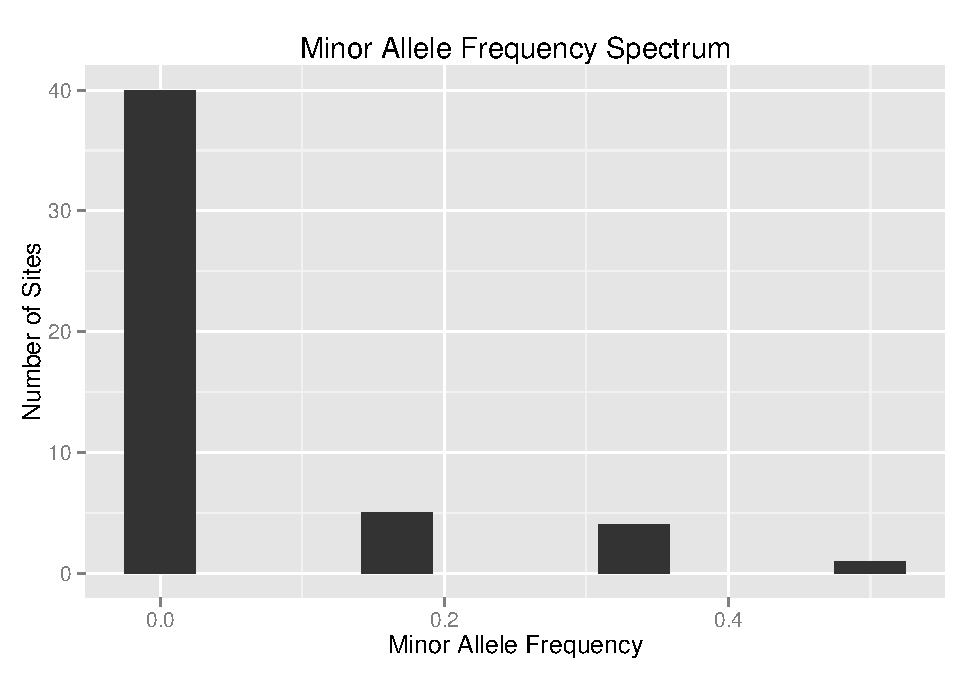
\includegraphics{munjal-201d-ps1_files/figure-latex/unnamed-chunk-27-1.pdf}
\pagebreak

\subsection{What is the derived allele frequency spectrum for these
data?}\label{what-is-the-derived-allele-frequency-spectrum-for-these-data}

\begin{Shaded}
\begin{Highlighting}[]
\NormalTok{sfsdata <-}\StringTok{ }\KeywordTok{matrix}\NormalTok{(}\OtherTok{NA}\NormalTok{,}\DecValTok{6}\NormalTok{,}\DecValTok{2}\NormalTok{)}
\KeywordTok{colnames}\NormalTok{(sfsdata) <-}\StringTok{ }\KeywordTok{c}\NormalTok{(}\StringTok{"DerivedAlleleFrequency"}\NormalTok{,}\StringTok{"NumberofSites"}\NormalTok{)}
\NormalTok{sfsdata[,}\DecValTok{2}\NormalTok{] <-}\StringTok{ }\KeywordTok{c}\NormalTok{(}\DecValTok{40}\NormalTok{,}\DecValTok{4}\NormalTok{,}\DecValTok{2}\NormalTok{,}\DecValTok{1}\NormalTok{,}\DecValTok{2}\NormalTok{,}\DecValTok{1}\NormalTok{)}
\NormalTok{sfsdata[,}\DecValTok{1}\NormalTok{] <-}\StringTok{ }\KeywordTok{c}\NormalTok{(}\DecValTok{0}\NormalTok{,}\DecValTok{1}\NormalTok{/}\DecValTok{6}\NormalTok{,}\DecValTok{2}\NormalTok{/}\DecValTok{6}\NormalTok{,}\DecValTok{3}\NormalTok{/}\DecValTok{6}\NormalTok{,}\DecValTok{4}\NormalTok{/}\DecValTok{6}\NormalTok{,}\DecValTok{5}\NormalTok{/}\DecValTok{6}\NormalTok{)}
\NormalTok{sfsdata}
\end{Highlighting}
\end{Shaded}

\begin{verbatim}
##      DerivedAlleleFrequency NumberofSites
## [1,]              0.0000000            40
## [2,]              0.1666667             4
## [3,]              0.3333333             2
## [4,]              0.5000000             1
## [5,]              0.6666667             2
## [6,]              0.8333333             1
\end{verbatim}

\begin{Shaded}
\begin{Highlighting}[]
\KeywordTok{library}\NormalTok{(ggplot2)}
\NormalTok{sfsdata <-}\StringTok{ }\KeywordTok{data.frame}\NormalTok{(sfsdata)}
\KeywordTok{qplot}\NormalTok{(}\DataTypeTok{x=}\NormalTok{sfsdata$DerivedAlleleFrequency,}\DataTypeTok{y=}\NormalTok{sfsdata$NumberofSites,}\DataTypeTok{geom=}\StringTok{"bar"}\NormalTok{,}
      \DataTypeTok{stat=}\StringTok{"identity"}\NormalTok{,}\DataTypeTok{width=}\FloatTok{0.05}\NormalTok{,}\DataTypeTok{xlab=}\StringTok{"Derived Allele Frequency"}\NormalTok{,}\DataTypeTok{ylab=}\StringTok{"Number of Sites"}\NormalTok{,}
      \DataTypeTok{main=}\StringTok{"Derived Allele Frequency Spectrum"}\NormalTok{)   }
\end{Highlighting}
\end{Shaded}

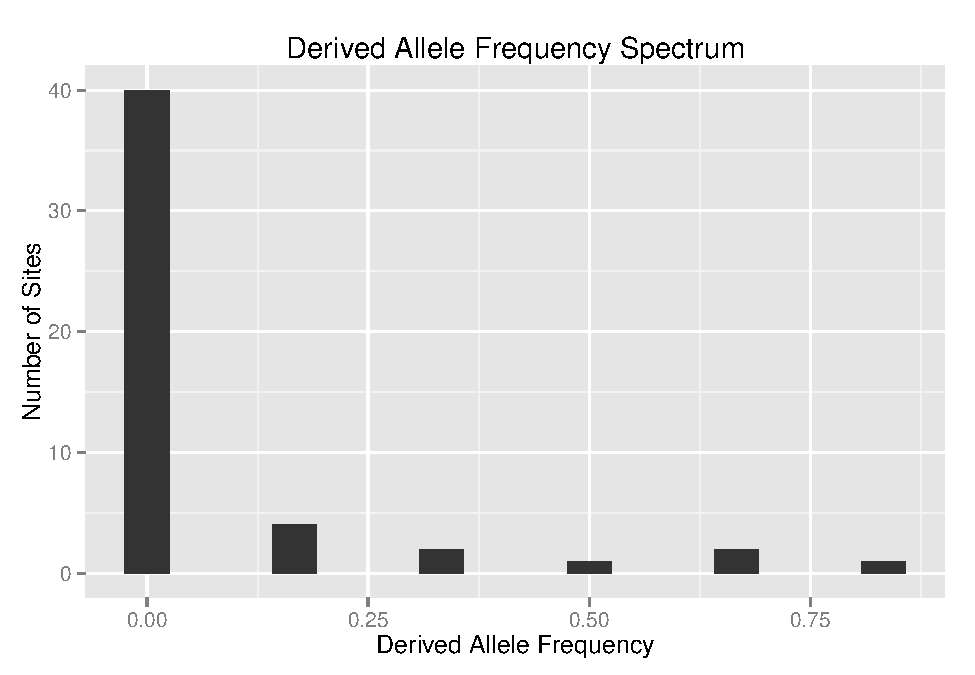
\includegraphics{munjal-201d-ps1_files/figure-latex/unnamed-chunk-28-1.pdf}

\end{document}
